\RequirePackage{etex}
\RequirePackage{tikz}

\documentclass[
	%draft,
	utf8,%     More capable input encoding than latin-1.
	parskip,%  For vertical whitespace between paragraphs.  This comes down to more than just using parskip.sty, so it's better to use this class option.
	% S5MP % If you intend to really use margin paragraphs (not recommended!).
	crop,%     Produce output with crop marks and paper size A4.  Liu-Tryck should like this.  Automatically adds information, including the physical page number, at the top of each page.
	%     Add option 'noInfo' to suppress the info at the top of each page when using option 'crop'.
	% Font options: 'kp' (default), 'times', 'lm'.  The KpFonts (loaded using 'kp'), is the most complete font among the provided options.  Among other, it supports slanted small caps.  See rtthesis.cls for more details regarding the font options.
	largesmallcaps,intlimits,widermath,% Good options to KpFonts.
	sharecounter,nobreak,definition=marks,%  See comments in the results chapter of this document for more information on these options!
	%article,
	numbers,% If you want to cite references by numbers, use this option.
	noparts% Use option 'noparts' if you do not make use of part divisions.	
]{rtthesis}

\usepackage{pgfplots}
\pgfplotsset{compat=1.12}
\usepgfplotslibrary{units}
\apptocmd{\sloppy}{\hbadness 10000\relax}{}{}

\usepackage{standalone}
\usepackage{mythesis}
\usepackage{multirow}
\usepackage{listings}
\usepackage{framed}
\usepackage{tablefootnote}
\usepackage{algorithm}
\usepackage{algpseudocode}
\usepackage{mathtools}
\usepackage[smallcaps, toc, nomain]{glossaries}
\usetikzlibrary{fit,positioning,arrows,arrows.meta,patterns}

\tikzset{every fit/.append style=text badly centered}

\renewcommand*{\acronymtype}{acronym}
\newglossary[alg]{acronym}{acr}{acn}{\acronymname}

\DeclarePairedDelimiter{\ceil}{\lceil}{\rceil}

\newcommand{\CTALG}{Cooley-Tukey}
\newcommand{\NVCARD}{GeForce GTX 670}
\newcommand{\AMDCARD}{Radeon R7 R260X}
\newcommand{\INTELCPU}{Intel Core i7 3770K 3.5GHz CPU}
\newcommand{\CU}{CUDA}
\newcommand{\OCL}{OpenCL}
\newcommand{\GL}{OpenGL}
\newcommand{\DX}{DirectCompute}
\newcommand{\OMP}{OpenMP}
\newcommand{\CPP}{C/C++}
\newcommand{\CUFFT}{cuFFT}
\newcommand{\CLFFT}{clFFT}
\newcommand{\FFTW}{FFTW}

\newcommand{\code}{\texttt}

\newacronym{ILP}{ILP}{Instruction-Level Parallelism}
\newacronym{1D}{1D}{One-dimensional}
\newacronym{2D}{2D}{Two-dimensional}
\newacronym{3D}{3D}{Three-dimensional}
\newacronym{API}{API}{Application Programming Interface}
\newacronym{CPU}{CPU}{Central Processing Unit}
\newacronym{CUDA}{CUDA}{Compute Unified Device Architecture}
\newacronym{DFT}{DFT}{Discrete Fourier Transform}
\newacronym{DIF}{DIF}{Decimation-In-Frequency}
\newacronym{DIT}{DIT}{Decimation-In-Time}
\newacronym{DRAM}{DRAM}{Dynamic Random-Access Memory}
\newacronym{DWT}{DWT}{Discrete Wavelet Transform}
\newacronym{FFT}{FFT}{Fast Fourier Transform}
\newacronym{FFTW}{FFTW}{Fastest Fourier Transform in the West}
\newacronym{GPGPU}{GPGPU}{General-Purpose computing on Graphics Processing Units}
\newacronym{GPU}{GPU}{Graphics Processing Unit}
\newacronym{OpenCL}{OpenCL}{Open Computing Language}
\newacronym{OpenGL}{OpenGL}{Open Graphics Library}
\newacronym{HLSL}{HLSL}{High-Level Shading Language}
\newacronym{GLSL}{GLSL}{OpenGL Shading Language}
\newacronym{SM}{SM}{Streaming Multiprocessor}
\newacronym{OS}{OS}{Operating System}
\newacronym{VLIW}{VLIW}{Very Long Instruction Word-processor}
\newacronym{EBCOT}{EBCOT}{Embedded Block Coding with Optimized Truncation}
\newacronym{DCT}{DCT}{Discrete Cosine Transform}
\newacronym{FLOPS}{FLOPS}{Floating-point Operations Per Second}
\newacronym{OpenMP}{OpenMP}{Open Multi-Processing}
\newacronym{BLAS}{BLAS}{Basic Linear Algebra Subprograms}
\newacronym{FPGA}{FPGA}{Field-Programmable Gate Array}
\newacronym{ACL}{ACL}{AMD Compute Libraries}
\newacronym{HBM2}{HBM2}{High Bandwidth Memory}
\newacronym{HBM}{HBM}{High Bandwidth Memory}
\newacronym{GCN}{GCN}{Graphics Core Next}
\newacronym{RDP}{RDP}{Remote Desktop Protocol}
\newacronym{HPC}{HPC}{High-Performance Computing}
\newacronym{PTX}{PTX}{Parallel Thread Execution}

\newglossaryentry{kernel}
{
  name=kernel,
  description={A GPU program},
  plural=kernels
}
\newglossaryentry{thread}
{
  name=thread,
  description={A way for a program to split itself to many simultaneously running tasks},
  plural=threads
}
\newglossaryentry{block}
{
  name=block,
  description={A way to organize threads, a block is executed by a multiprocessing unit},
  plural=blocks
}

\makeglossaries

\begin{document}%
%
\selectlanguage{english}%
%\makeFrontPage%
\frontmatter%
\maketitle%
%\makeLibraryPage{The computational capacity of graphics cards for general-purpose computing have been progressing fast over the last decade. A major reason is demanding computer games, where standard of performance and high quality graphics are constantly raised. Another reason are better suitable technologies for programming the graphics cards. Combined, the product are high raw performance devices and means to access that performance. This thesis investigates some of the current technologies for general-purpose computing on graphics processing units. Technologies are primarily compared by means of benchmarking performance and secondarily by factors concerning programming and implementation. The selection of technology can have a large impact on performance. The benchmark application found the difference of the fastest technology, CUDA, compared to the slowest, OpenCL, to be twice as long execution time. The application also found out that the older technologies, OpenGL and DirectX, are competitive with CUDA and OpenCL in terms of the resulting performance speed.%151
%
%En sammanfattning ska kort och koncist beskriva och motivera det studerade problemet, metoden samt resultat och slutsatser. Arbetets bidrag till huvudområdet ska tydligt framgå. Vad är det rapporten säger om huvudområdet som vi inte visste tidigare? Exempel på bidrag kan vara vilken effekt en specifik algoritm eller programutvecklingsmetod får i en specifik tillämpning.
%
%Normalt ska en sammanfattning vara högst 150 ord, och inte innehålla några referenser eller radbrytningar.
%
%Sammanfattning på svenska såväl som engelska (abstract) måste finnas med. Om rapporten är skriven på engelska räcker det med engelsk sammanfattning }%
\begin{abstract}[english]%
	The computational capacity of graphics cards for general-purpose computing have been progressing fast over the last decade. A major reason is demanding computer games, where standard of performance and high quality graphics are constantly raised. Another reason are better suitable technologies for programming the graphics cards. Combined, the product are high raw performance devices and means to access that performance. This thesis investigates some of the current technologies for general-purpose computing on graphics processing units. Technologies are primarily compared by means of benchmarking performance and secondarily by factors concerning programming and implementation. The selection of technology can have a large impact on performance. The benchmark application found the difference of the fastest technology, CUDA, compared to the slowest, OpenCL, to be twice as long execution time. The application also found out that the older technologies, OpenGL and DirectX, are competitive with CUDA and OpenCL in terms of the resulting performance speed.%151
%
%En sammanfattning ska kort och koncist beskriva och motivera det studerade problemet, metoden samt resultat och slutsatser. Arbetets bidrag till huvudområdet ska tydligt framgå. Vad är det rapporten säger om huvudområdet som vi inte visste tidigare? Exempel på bidrag kan vara vilken effekt en specifik algoritm eller programutvecklingsmetod får i en specifik tillämpning.
%
%Normalt ska en sammanfattning vara högst 150 ord, och inte innehålla några referenser eller radbrytningar.
%
%Sammanfattning på svenska såväl som engelska (abstract) måste finnas med. Om rapporten är skriven på engelska räcker det med engelsk sammanfattning %
\end{abstract}%
\begin{acknowledgments}%
	I would like to thank Åsa Detterfelt for the opportunity to make this thesis work at MindRoad AB. I would also like to thank Ingemar Ragnemalm at ISY.
	
	\addvspace{1em}%
	\begin{flushright}%
    \textit{%
		Linköping, Februari 2016 \\%
		Torbjörn Sörman%
	}%
	\end{flushright}%
	
\end{acknowledgments}%
%
%
\tableofcontents%
\newpage%
\listoftables%
\newpage%
\listoffigures%
\newpage%
\printglossary[type=\acronymtype,nonumberlist]%
%\newpage%
%\printglossary[type=main,nonumberlist]%
%\begin{notation}% Passing the option "old" to the notation environment will redefine the notationtabular environment so that it produces an old style LaTeX tabular instead of a ctable.sty style tabular.
	\centering
	
	\begin{notationtabular}{Glossary}{Term}{Meaning}
		Kernel & A \gls{GPU} program \\
		Thread & A way for a program to split itself to many simultaneously running tasks \\
		Block & A way to organize threads, a block is executed by a multiprocessing unit \\
	\end{notationtabular}

\end{notation}
%
\mainmatter%
\chapter{Introduction}\label{cha:intro}
This chapter gives an introduction to the thesis. It describes the background, purpose and goal of the thesis, and also a list of abbreviations and the structure of this report.

\section{Background}
The computationally demanding problems have during a long period of time been solved faster by technical improvements in hardware. However, some limitations have been reached the last decades. Operating frequency of the \gls{CPU} is no longer significantly improved. Problems relying on single thread performance are limited by three primary technical factors:
\begin{enumerate}
	\item The \gls{ILP} wall
	\item The memory wall
	\item The power wall
\end{enumerate}

The first wall states that its hard to further exploit simultanious \gls{CPU} instructions, techniques like instruction pipelining, superscalar execution and \gls{VLIW} exists but complexity and latency of hardware reduces the benefits. Related to the first is second wall, the gap between \gls{CPU} speed and memory access time, that may cost several hundreds of \gls{CPU} cykles if accessing primary memory. The third wall is power and heating problem. The power consumed is increased exponentially with each factorial increase of operating frequency.

Improvements can be found in exploiting parallelism. Either reconstruct the problem or the problem itself is already inherently parallelizable. This trend manifests in development towards use and construction of multi-core microprocessors. The \gls{GPU} is one such device, originally exploited the inherent parallelism within visual rendering but now is available as a tool for massively parallelizable problems.

\section{Problem statement}
Programmers might experience a threshold and slow learning curve to move from sequential to thread-parallel programming that is \gls{GPU} programming. Obstacles involve learning about the hardware architecture and restructure the application. Knowing limitations and benefits might even provide reason to not utilize the \gls{GPU} and instead choose to work with a multi-core \gls{CPU}.

Depending on one's preferences, needs and future goals; selecting one technology over the other might be derived from portability or hardware requirements, programmability, how well it integrates with other frameworks or \gls{API} or how well it's supported by the provider or developer community. Within the range of this thesis, the covered technologies are \gls{CUDA}, \gls{OpenCL}, DirectCompute (\gls{API} within DirectX) and \gls{OpenGL} Compute Shaders.

\section{Purpose and goal of the thesis work}
One goal is to evaluate, select and implement an application suitable for \gls{GPGPU}.

Implement the same application in important technologies for \gls{GPGPU}:
\begin{itemize}
	\item \CU
	\item \OCL
	\item \DX
	\item \GL
\end{itemize}
Compare results with sequential {\CPP} implementation and an multi-core {\OMP} implementation.

The purpose is to compare the different technologies by means of benchmarking performance and make relevant qualitative assessments.%
\chapter{Benchmark algorithm}
This part cover some possible applications for a GPGPU study. The basic theory and motivation why they are suitable for benchmarking GPGPU technologies is presented. For this thesis, the Fast Fourier Transform is selected as the benchmarking application and will be more detailed in another part of the report.

\newtheorem{thm}{Theorem}[chapter] % reset theorem numbering for each chapter
\theoremstyle{definition}
\newtheorem{defn}[thm]{Definition} 

\section{Discrete Fourier Transform}
The Fourier transform is of use when analysing the spectrum of a continuous analogue signal. When applying transformation to a signal it is decomposed into the frequencies that makes it up. In digital signal analysis the Discrete Fourier transform (DFT) is the counterpart of the Fourier transform for analogue signals. The DFT converts a sequence of finite length into a list of coefficients of a finite combination of complex sinusoids. Given that the sequence is a sampled function from the time or spatial domain it's a conversion to the frequency domain. It is defined as
\begin{equation}
	X_k=\sum_{n=0}^{N-1}x(n)W_N^{kn}, k \in {[0, N-1]}	
\end{equation}
where $W_N^{kn}=e^{-2iknN}$, commonly named the twiddle factor\cite{Gentleman1966}.

The DFT is used in many practical applications to perform Fourier analysis. In digital signal processing, such as discrete samples of sound waves, radio signal or any continuous signal over a finite time interval. In image processing the sampled sequence can be pixels along a row or column. The DFT takes input in complex numbers and outputs in complex coefficients. In practical applications the input is usually real numbers.

\subsection{Fast Fourier Transform}
The problem with the DFT is that it has by definition a time complexity of $\mathcal{O}(n^n)$ that makes it too slow for some applications. The Fast Fourier Transform (FFT) is one of the most common algorithm used to compute the DFT of a sequence. An FFT computes the transformation by factorizing the transformation matrix of the DFT into a product of mostly zero factors. This reduces the time complexity to $\mathcal{O}(n\log{}n)$.
The FFT was made popular in 1965 by J.W Cooley and J.W. Tukey and it found its way into practical use at the same time and meant a serious breakthrough in digital signal processing \cite{Cooley1969, Brigham1967}. However the complete algorithm was not invented at the time, the history of the Cooley-Tukey FFT algorithm can be traced back to around 1805 by work of the famous mathematician Carl Friedrich Gauss\cite{Heideman1985}.

The algorithm is a divide and conquer algorithm that relies on recursively dividing the input into sub-blocks and eventually the problem is small enough to be solved and the sub-blocks are combined into the final result.
\section{Image processing}
Image processing consists of a wide range of domains. Earlier academic work with performance evaluation on the GPU\cite{Park2011} tested four major domains (3D shape reconstruction, feature extraction, image compression and computational photography) and compared with the CPU. Generally image processing is by nature parallel and one can expect good results on a GPU.

Most of image processing algorithms apply the same computation on a number of pixels and that is a typically data parallel operation. Some algorithms can then be expected to have huge speed up compared to an efficient CPU implementation. A representative task is applying a simple image filter that gathers neighboring pixel-values and compute a new value for a pixel. If done with respect to the underlying structure of the system one can expect a speedup near linear to the number of computational cores used. That is a CPU with four cores can theoretically expect a near four time speedup compared to a single core. This extends to a GPU so a GPU with n cores can in ideal cases expect a speedup in the order of n. An example of this is a Gaussian blur (or smoothing) filter.

\section{Image compression}
The image compression standard JPEG2000 offers algorithms with parallelism but is very computationally and memory intensive. The standard aims to improve performance over JPEG but also adding new features. The following sections are part of the JPEG2000 algorithm\cite{Christopoulos2000}.
\begin{enumerate}
	\item Color Component transformation
	\item Tiling
	\item Wavelet transform
	\item Quantization
	\item Coding
\end{enumerate}

The computation heavy parts can be identified as the Discrete Wavelet Transform (DWT) and the encoding engine using Embedded Block Coding with Optimized Truncation (EBCOT) Tier-1.

The important difference between the older format JPEG compared to JPEG2000 is the use of DWT instead of Discrete Cosine Transform (DCT). In comparison to the DFT, the DCT operates solely on real values but at the same time complexity. DWT's on the other hand uses another representation that allows for a time complexity of $\mathcal{O}(N)$.

\section{Linear algebra}
Linear algebra is central to both pure and applied mathematics. In scientific computing it's a highly relevant problem to solve dense linear systems efficiently. From the initial uses of GPUs in scientific computing the graphics pipeline was successfully used for linear algebra through programmable vertex and pixel shaders\cite{Kruger2003}. Later on methods and systems for utilizing GPUs have been shown efficient also in hybrid system (multi-core CPUs + GPUs)\cite{Tomov2010}. Linear algebra is highly suitable for GPUs and with careful calibration it is possible to reach 80\%-90\% of the theoretical peak speed of large matrices\cite{Volkov2008}.

Common operations are vector addition, scalar multiplication, dot products, linear combinations, and matrix multiplication. Matrix multiplications are of much interest since the high time complexity $\mathcal{O}(N^3)$ makes it a bottleneck in many algorithms. Matrix decomposition like LU, QR and Cholesky decomposition are used very often and are subject for benchmarking GPUs to linear algebra\cite{Volkov2008}.

\section{Sorting}
The sort operation is an important part in computer science and have been a classic problem to work on. There exists several techniques and mostly it comes down to what problem you have and choose the best suited algorithm.

Sorting algorithms can be organized into two categories, data-driven and data-independent. The classic quicksort algorithm is probably the best known example of a data-driven sorting algorithm. It performs with time complexity On log(n) on average but have a time complexity of ON2 in the worst case. Another data-driven algorithm that does not have this problem is heap sort but instead it suffers from difficult data access patterns. Data-driven algorithms are not the easiest to parallelize since the behaviour is unknown and may cause bad load balancing.

The other category are the algorithms that always perform the same process no matter what the data. This behaviour makes suitable for implementation on multiple processors, fixed sequences of instructions where the moment in which data is synchronized and communication must occur are known in advance.

\subsection{Efficient sorting}
Bitonic sort have been used early on in the utilization of GPUs for sorting, even though it has the time complexity of On log(n2) it's been an easy way of doing reasonably efficient sort on GPUs. Other high performance sorting on GPUs are often combinations of algorithms. Examples of fast sorting algorithms on GPUs have used bucket sort or quicksort that first splits the list into sublist and then sort in parallel with merge sort or by using bitonic sort followed by merge sort.

A popular algorithm for GPUs have been variants of radix sort which is a non-comparative integer sorting algorithm. Radix sorts can be described as being easy to implement and still as efficient as more sophisticated algorithms. Radix sort works by grouping the integer keys by the individual digits value in the same significant position and value.

\section{Criteria for Algorithm Selection}
For this thesis, a benchmarking application is sought after that have the necessary complexity and relevance to both practical uses and the scientific community. The algorithm with enough complexity and challenges is the FFT, compared to the other presented algorithms the FFT are more complex than the matrix operations and the regular sorting algorithms. The FFT does not demand as much domain knowledge as the image compression algorithms but its still a very potent algorithm for many specific applications.

The major difficulties working with multi-core systems are applied to GPUs. What GPUs are missing compared to multi-core CPUs are the power of working in sequential, instead GPUs are excellent at fast context switching and hiding memory latencies. Most effort of working with GPUs must be to put into supply with enough parallelism, avoiding branching and refine memory access patterns. One important issue is also the host to device memory transfer-time. If the algorithm is much faster on the GPU, a CPU could still be faster if the host to device and back transfer is a large part of the total time.
By selecting an algorithm that have much scientific interest and history; relevant comparisons can be made and it is sufficient to say that one can demand a reasonable performance by utilizing information sources concerning other implementations on GPUs. 

%
\chapter{Theory}

This chapter will give an introduction to the FFT algorithm and a brief introduction of the Graphics Processing Unit (GPU).

\section{Graphics Processing Unit}

A GPU is traditionally specialized hardware for efficient manipulation of computer graphics and image processing. The inherent parallel structure of images and graphics makes them very efficient at some more general problems where parallelism can be exploited. The concept of General-purpose computing on graphics processing units (GPGPU) is solving a problem on the GPU platform instead of a multi-core CPU system.

\subsection{GPGPU}

In the early days of GPGPU one had to know a lot about computer graphics to compute general data. The available APIs was created for graphics processing. The dominant APIs was OpenGL and DirectX. HLSL (High Level Shader Language) and GLSL (OpenGL Shader Language) made the step easier but it still generated code into the APIs.

A big change was when NVIDIA released {\CU} and together with new hardware made it possible to use standard C-code to program the GPU (with a few extensions). The fact that parallel software and hardware was a small market at the time, the simplified use of the GPU for parallel tasks opened up to many more customers. However, the main business is still graphics and the manufacturers can not make cards too expensive, especially at the cost of graphics performance (as integrating more double precision capacity would). This can be exemplified with the release of NVIDIA's Maxwell micro architecture, compared to the predecessor Kepler, both are similar but with Maxwell some of the double precision support was removed in favour of single precision (used in graphics).

\subsection{GPU vs CPU}

The GPU is built on a principle of more execution units instead of higher clock-frequency to improve performance. Comparing the CPU with the GPU, the GPU performs a much higher floating point operations per second (FLOP) if running at optimal conditions. The GPU relies on using high memory bandwidth and fast context switching (run the next warp of threads) to compensate for lower frequency and hide memory latencies. The CPU is excellent at sequential tasks with features like branch prediction that can not be found on the GPU.

The GPU thread is very lightweight and its creation have very little overhead, whereas on the CPU the thread can be seen as an abstraction of the processor and switching a thread is considered expensive since the context have to be loaded each time. On the other hand, a GPU is very inefficient if not enough threads are ready to work. Memory latencies are supposed to be hidden by switching in a new set of working threads as fast as possible.

A CPU thread have its own registers but the GPU thread work in groups where they share registers and memory. One can not give individual instructions to each thread, all of them will execute the same instruction. The figure \ref{fig:gpu-vs-cpu} demonstrates this by showing that by sharing control-structure and cache, the GPU puts more resources on processing then the CPU where more resources goes into control structures and memory cache.

\begin{figure}
	\centering
	\includestandalone[width=\textwidth]{figures/gpu-cpu}
	\caption{The GPU uses more transistors for data processing}
	\label{fig:gpu-vs-cpu}
\end{figure}

\section{Fast Fourier Transform}

This section extends the information from section \ref{sec:algorithms:fft} in the \textit{Benchmark application} chapter.

\subsection{\CTALG}

The Fast Fourier Transform is by far mostly associated with the {\CTALG} algorithm. The {\CTALG} algorithm is a devide and conquer algorithm that recursively breaks down a DFT of any composite size of $N = N_1{\cdot}N_2$. The algorithm decomposes the DFT into $s = \log_r{N}$ stages. The $N$-point DFT is composed of $r$-point small DFTs in $s$ stages. In this context the $r$-point DFT is called radix-$r$ butterfly.

\subsubsection{Butterfly and radix-2}

The implementation of a $N$-point radix-2 FFT algorithm have $\log_2{N}$ stages with $N/2$ butterfly operations per stage. A butterfly operation is an addition, a subtraction, followed by a multiplication by a twiddle factor, see figure \ref{fig:butterfly}.

\begin{figure}
	\centering
	% FFT Butterfly
\tikzstyle{n}= [circle, fill, minimum size=4pt,inner sep=0pt, outer sep=0pt]
\tikzstyle{mul} = [circle,draw,inner sep=-1pt, minimum size=7pt]
\tikzstyle{sub} = [circle,draw,inner sep=-1pt, minimum size=7pt]
\tikzstyle{add} = [circle,draw,inner sep=-1pt, minimum size=7pt]

\begin{tikzpicture}[
	yscale=1.3,
	xscale=1.8,
	node distance=0.7cm,
	auto]
    
	\node[n, pin={[pin edge={latex'-,black}]left:$x(0)$}] (N-0-0) at (0,-0) {};
	\node[n, pin={[pin edge={latex'-,black}]left:$x(1)$}] (N-0-1) at (0,-1) {};
                            
	\node[add, name=N-1-0, pin={[pin edge={-latex',black},pin distance=1.175cm]right:$X(0)$}] at (1,-0) {${+}$};
	\node[sub, name=N-1-1, label={[label distance=-10pt]90:${-}$}] at (1,-1) {};
            
	\node[mul, right of=N-1-1, label={above right:\tiny $W^{k}_{N}$},
		pin={[pin edge={-latex',black}]right:$X(1)$}] (N-2-1) {${\times}$};       

	\path (N-0-0) edge[-latex'] (N-1-0);	
	\path (N-0-1) edge[-latex'] (N-1-1);
	\path (N-1-1) edge[-latex'] (N-2-1);
      
    % Connect nodes
    \foreach \src / \dst in {	0/0, 0/1, 1/0, 1/1}
       \path (N-0-\src.east) edge[-latex'] (N-1-\dst.west);
       
\end{tikzpicture}
	\caption{Radix-2 butterfly operations}
	\label{fig:butterfly}
\end{figure}

Figure \ref{fig:cooley-tukey-8} shows an 8-point radix-2 DIF FFT. The input are in natural order whereas the output are in bit reversed order.

\begin{figure}
	\centering
	% FFT Butterfly
\tikzstyle{n}= [circle, fill, minimum size=4pt,inner sep=0pt, outer sep=0pt]
\tikzstyle{mul} = [circle,draw,inner sep=-1pt]

% Define two helper counters
\newcounter{x}\newcounter{y}
\begin{tikzpicture}[%
	%yscale=0.6,
	%xscale=1.2,
	node distance=0.25cm,
	auto]
    % Draw inputs
    \foreach \y in {0,...,7}
        \node[n, pin={[pin edge={latex'-,black}]left:$x(\y)$}] (N-0-\y) at (0,-\y) {};

	\foreach \y in {0,...,7}
        \foreach \x / \c in {1/1,2/3,3/4,4/6,5/7,6/9}
            \node[n, name=N-\c-\y] at (\x,-\y) {};           
    
    % Draw outputs
    \foreach \y in {0,...,7}
        \node[n, pin={[pin edge={-latex',black}]right:$X(\y)$}] (N-11-\y) at (8,-\y) {};
        
    % horizontal connections
    % Note the use of simple counter arithmetics to get correct
    % indexes.
    \foreach \y in {0,...,15}
    {
		\foreach \x in {0,1,3,4,7}
		{
			\setcounter{x}{\x}\stepcounter{x}
			\path (N-\x-\y) edge[-] (N-\arabic{x}-\y);
		}
	}
           
    % Draw the W_8 coefficients
    \setcounter{y}{0}
    \foreach \tmp in {0,1}
	{
    	\foreach \i in {0,...,3}
    	{
        	\path (N-5-\arabic{y}) edge[-] node {} (N-6-\arabic{y});
        	\addtocounter{y}{1}
    	}
    }

    % Draw the W_4 coefficients
    \setcounter{y}{0}
    \foreach \tmp in {0,1}
	{
    	\foreach \i in {0,1}
    	{
        	\path (N-5-\arabic{y}) edge[-] node {} (N-6-\arabic{y});
        	\addtocounter{y}{1}
    	}
    	\foreach \i in {0,1}
    	{
        	\path (N-5-\arabic{y}) edge[-] node {\tiny $W^{\i}_{8}$} (N-6-\arabic{y});
        	\addtocounter{y}{1}
    	}
    }
    
    % Connect nodes
    \foreach \sourcey / \desty in {	0/4,	1/5,	2/6,	3/7,
									4/0,	5/1,	6/2,	7/3}
        \path (N-3-\sourcey.east) edge[-] (N-4-\desty.west);
    \foreach \sourcey / \desty in {	0/0,	1/2,	2/0,	3/2,
    								0/1,	1/3,	2/1,	3/3,
                                   	4/4,	5/6,	6/4,	7/6,
                                   	4/5,	5/7,	6/5,	7/7,}
	{
        \path (N-6-\sourcey.east) edge[-] (N-7-\desty.west);
        \path (N-9-\sourcey.east) edge[-] (N-10-\desty.west);
    }
    
    % Add region boxes	
    % Complete stage
	\node[draw,densely dotted,fit=(N-0-0) (N-2-15),label=above:{stage 1}] {};
	\node[draw,densely dotted,fit=(N-3-0) (N-5-15),label=above:{stage 2}] {};
	\node[draw,fit=(N-6-0) (N-8-15),opacity=0,label=above:{stage 3},name=Stage-3] {};
	\node[draw,fit=(N-9-0) (N-\lastNode-15),opacity=0,label=above:{stage 4},name=Stage-4] {};
	\node[draw,fit=(N-11-0) (N-11-15),opacity=0,label=above:{output}] {};
	\node[draw,densely dotted,fit=(Stage-3) (Stage-4)] {};
	\node[draw,fit=(N-\lastNode-0) (N-11-15)] {};
\end{tikzpicture}
	\caption{8-point radix-2 FFT using {\CTALG} algorithm}
	\label{fig:cooley-tukey-8}
\end{figure}

\subsubsection{\CGALG}

Similar to {\CTALG} but with another data access pattern that uses the same indexing in all stages. This removes the overhead of calculating the data input index at each stage as in figure \ref{fig:cooley-tukey-8} where the top butterfly first stage require input $x[0], x[4]$ and in the second stage $x[0], x[2]$ whereas using the {\CGALG} algorithm in figure \ref{fig:constant-geometry-8} the equivalent input are $x[0], x[4]$ for all stages.

\begin{figure}
	\centering
	% FFT Butterfly
\tikzstyle{n}= [circle, fill, minimum size=4pt,inner sep=0pt, outer sep=0pt]
\tikzstyle{mul} = [circle,draw,inner sep=-1pt]

% Define two helper counters
\newcounter{x}\newcounter{y}
\begin{tikzpicture}[%
	yscale=0.6,
	xscale=1.2,
	node distance=0.25cm,
	auto]
    % The strategy is to create nodes with names: N-column-row
    % Input nodes are named N-0-0 ... N-0-15
    % Output nodes are named N-10-0 ... N-10-15

    % Draw inputs
    \foreach \y in {0,...,15}
        \node[n, pin={[pin edge={latex'-,black}]left:$x(\y)$}] (N-0-\y) at (0,-\y) {};
              
    % Draw outputs
    \foreach \y in {0,...,15}
        \node[n, pin={[pin edge={-latex',black}]right:$X(\y)$}] (N-11-\y) at (8,-\y) {};
              
   % draw connector nodes
    \foreach \y in {0,...,15}
        \foreach \x / \c in {1/1,2/3,3/4,4/6,5/7,6/9,7/10}
            \node[n, name=N-\c-\y] at (\x,-\y) {};
            
    % draw x nodes
    \foreach \y in {0,...,7}
        \foreach \x / \c  in {1/2}
            \node[mul, right of=N-\x-\y] (N-\c-\y) {};            
    \foreach \y in {8,...,15}
        \foreach \x / \c  in {1/2}
            \node[mul, right of=N-\x-\y] (N-\c-\y) {${\times}$};
    % 
    \foreach \y in {0,...,3}
        \foreach \x / \c  in {4/5}
            \node[mul, right of=N-\x-\y] (N-\c-\y) {};
    \foreach \y in {4,...,7}
        \foreach \x / \c  in {4/5}
            \node[mul, right of=N-\x-\y] (N-\c-\y) {${\times}$};
    \foreach \y in {8,...,11}
        \foreach \x / \c  in {4/5}
            \node[mul, right of=N-\x-\y] (N-\c-\y) {};
    \foreach \y in {12,...,15}
        \foreach \x / \c  in {4/5}
            \node[mul, right of=N-\x-\y] (N-\c-\y) {${\times}$};
    % 
    \foreach \y in {0,2,4,6,8,10,12,14}
        \foreach \x / \c  in {7/8}
            \node[mul, right of=N-\x-\y] (N-\c-\y) {};
    \foreach \y in {1,3,5,7,9,11,13,15}
        \foreach \x / \c  in {7/8}
            \node[mul, right of=N-\x-\y] (N-\c-\y) {${\times}$};    

    % horizontal connections
    % Note the use of simple counter arithmetics to get correct
    % indexes.
    \foreach \y in {0,...,15}
    {
		\foreach \x in {0,1,3,4,7}
		{
			\setcounter{x}{\x}\stepcounter{x}
			\path (N-\x-\y) edge[-] (N-\arabic{x}-\y);
		}
	}
       
    % Draw the W_16 coefficients
    \setcounter{y}{0}
    \foreach \i in {0,...,7}
    {
	   	\path (N-2-\arabic{y}) edge[-] node {} (N-3-\arabic{y});
	    \stepcounter{y}
    }
    \foreach \i in {0,...,7}
    {
    	\path (N-2-\arabic{y}) edge[-] node {\tiny $W^{\i}_{16}$} (N-3-\arabic{y});
        \stepcounter{y}
    }
    
    % Draw the W_8 coefficients
    \setcounter{y}{0}
    \foreach \tmp in {0,1}
	{
    	\foreach \i in {0,...,3}
    	{
        	\path (N-5-\arabic{y}) edge[-] node {} (N-6-\arabic{y});
        	\addtocounter{y}{1}
    	}
    	\foreach \i in {0,...,3}
    	{
        	\path (N-5-\arabic{y}) edge[-] node {\tiny $W^{\i}_{8}$} (N-6-\arabic{y});
        	\addtocounter{y}{1}
    	}
    }

    % Draw the W_4 coefficients
    \setcounter{y}{0}
	\foreach \tmp in {0,...,3}
	{    
		\foreach \i in {0,1}
		{
			\path (N-8-\arabic{y}) edge[-] node {} (N-9-\arabic{y});
			\stepcounter{y}
			\path (N-8-\arabic{y}) edge[-] node {\tiny $W^{\i}_{4}$} (N-9-\arabic{y});
			\stepcounter{y}
		}
    }
    
    % Connect nodes
    \foreach \sourcey / \desty in {	0/8,	1/9,	2/10,	3/11,
									4/12,	5/13,	6/14,	7/15,
									8/0,	9/1,	10/2,	11/3,
									12/4,	13/5,	14/6,	15/7}
       \path (N-0-\sourcey.east) edge[-] (N-1-\desty.west);
    \foreach \sourcey / \desty in {	0/4,	1/5,	2/6,	3/7,
									4/0,	5/1,	6/2,	7/3,
									8/12,	9/13,	10/14,	11/15,
									12/8,	13/9,	14/10,	15/11}
        \path (N-3-\sourcey.east) edge[-] (N-4-\desty.west);
    \foreach \sourcey / \desty in {	0/0,	1/2,	2/0,	3/2,
    								0/1,	1/3,	2/1,	3/3,
                                   	4/4,	5/6,	6/4,	7/6,
                                   	4/5,	5/7,	6/5,	7/7,
                                   	8/8,	9/10,	10/8,	11/10,
									8/9,	9/11,	10/9,	11/11,
									12/12,	13/14,	14/12,	15/14,
									12/13,	13/15,	14/13,	15/15}
	{
        \path (N-6-\sourcey.east) edge[-] (N-7-\desty.west);
        \path (N-9-\sourcey.east) edge[-] (N-10-\desty.west);
    }
    % Nodes are in bit-reverse order
    \foreach \sourcey / \desty in {	0/0,1/8,2/4,3/12,4/2,5/10,6,7/14,8/1,9,10/5,11/13,12/3,13/11,14/7,15/15}
	{
        \path (N-10-\sourcey.east) edge[-] (N-11-\desty.west);
    }
    
    % Add region boxes
	% Partial stage
	\def \lastNode {10}
	\node[draw,dashed,fit=(N-6-0) (N-\lastNode-3)] {};
	\node[draw,dashed,fit=(N-6-4) (N-\lastNode-7)] {};
	\node[draw,dashed,fit=(N-6-8) (N-\lastNode-11)] {};
	\node[draw,dashed,fit=(N-6-12) (N-\lastNode-15)] {};	
    % Complete stage
	\node[draw,densely dotted,fit=(N-0-0) (N-2-15),label=above:{stage 1}] {};
	\node[draw,densely dotted,fit=(N-3-0) (N-5-15),label=above:{stage 2}] {};
	\node[draw,fit=(N-6-0) (N-8-15),opacity=0,label=above:{stage 3},name=Stage-3] {};
	\node[draw,fit=(N-9-0) (N-\lastNode-15),opacity=0,label=above:{stage 4},name=Stage-4] {};
	\node[draw,fit=(N-11-0) (N-11-15),opacity=0,label=above:{output}] {};
	\node[draw,densely dotted,fit=(Stage-3) (Stage-4)] {};
	\node[draw,fit=(N-\lastNode-0) (N-11-15)] {};
\end{tikzpicture}
	\caption{8-point radix-2 FFT using {\CGALG} algorithm}
	\label{fig:constant-geometry-8}
\end{figure}

\subsection{Parallelism in FFT}

By examining the FFT algorithm, parallelism can be exploited in several ways. Naturally when decomposing the DFT into radix-2 operations, parallelism can be achieved by mapping one thread per data input. That would however lead to unbalanced load as every second input is multiplied by the complex twiddle factor whereas the other is not. By selecting one thread per radix-2 butterfly operation instead, each thread will share the same workload.

\subsection{GPU algorithm}

The complete FFT application can be implemented in two different kernels, one kernel executing over a single stage and one kernel executing the last stages that could fit within one block. The single-stage kernel, called \emph{global kernel}, would execute in sequential order each stage of the algorithm. Each execution would require in total as many threads as there are butterfly-operations. The host would supply the kernel with arguments depending on stage and problem size. See table \ref{tab:global-kernel} for full parameter list. The global kernel algorithm is shown in \ref{alg:device:global-kernel}. The global kernel would only be called for the number of stages not fitted in a single block (this depends on selected number of threads per block). The global kernel implements {\CTALG} algorithm.

\begin{table}
	\centering
	\begin{tabular}{|l|l|}
		\hline
		Parameter & Argument \\ \hline
		\textit{data} & Input/Output data buffer \\ \hline
		\textit{stage} & $[0,\log_{2}(N) - \log_{2}(N_{block})]$ \\ \hline
		\textit{bitmask} & $\Call{LeftShift}{\texttt{FFFFFFFF}_{16}, 32 - stage}$ \\ \hline
		\textit{angle} & $(2 \cdot \pi)/N$ \\ \hline
		\textit{dist} & $\Call{RightShift}{N, steps}$ \\ \hline		
	\end{tabular}
	\caption{Global kernel parameter list with argument depending on size of input $N$ and $stage$.}
	\label{tab:global-kernel}
\end{table}

\begin{algorithm}
	\centering
	\begin{algorithmic}[1]
		\Procedure{GlobalKernel}{$data, stage, bitmask, angle, dist$}
            \State $tid \gets \Call{GlobalThreadId}{}$ 
            \State $low \gets tid + (tid \And bitmask)$
            \State $high \gets low + dist$
            \newline
            %\State // Calculate twiddle-factor
            \State $twMask \gets \Call{ShiftLeft}{dist - 1, stage}$
            \State $twStage \gets \Call{PowerOfTwo}{stage} \cdot tid$
            \State $a \gets angle \cdot (twStage \And twMask)$
            \State $\Call{Imag}{twiddleFactor} \gets \Call{Sin}{a}$
            \State $\Call{Real}{twiddleFactor} \gets \Call{Cos}{a}$
            \newline
            %\State // Calculate butterfly-operations
            \State $temp \gets \Call{ComplexSub}{data_{low}, data_{high}}$
            \State $data_{low} \gets \Call{ComplexAdd}{data_{low}, data_{high}}$
            \State $data_{high} \gets \Call{ComplexMul}{temp, twiddleFactor}$
        \EndProcedure
	\end{algorithmic}
	\caption{Pseudo-code for the global kernel with input from the host.}
	\label{alg:device:global-kernel}
\end{algorithm}

\subsubsection{Shared/Local memory}

The \textit{local kernel} is always called and encapsulates all remaining stages and the bit reverse order output procedure. It is devised as to utilize shared memory completely for all stages. This reduces the primary memory access to read input and write output. The kernel implements the {\CGALG} algorithm to increase performance in the inner loop, the input and output index is calculated once. See algorithm \ref{alg:device:local-kernel}.

\begin{table}
	\centering
	\begin{tabular}{|l|l|}
		\hline
		Parameter & Argument \\ \hline
		\textit{in} & Input data buffer \\ \hline
		\textit{out} & Output data buffer \\ \hline
		\textit{angle} & $(2 \cdot \pi)/N$ \\ \hline
		\textit{stages} & $[\log_{2}(N) - \log_{2}(N_{block}), \log_{2}(N)]$ \\ \hline
		\textit{leadingBits} & $32 - \log_{2}(N)$ \\ \hline
		\textit{c} & Forward: $-1$, Inverse: $1/N$ \\ \hline
	\end{tabular}
	\caption{Local kernel parameter list with argument depending on size of input $N$ and number of stages left to complete.}
	\label{tab:local-kernel}
\end{table}

\begin{algorithm}
	\centering
	\begin{algorithmic}[1]
		\Procedure{LocalKernel}{$in$, $out$, $angle$, $stages$, $leadingBits$, $c$}
            \State let $shared$ be a shared/local memory buffer     
            \State $low  \gets \Call{ThreadId}{}$
            \State $high \gets low + \Call{BlockDim}{}$   
            \State $offset \gets \Call{BlockId}{} \cdot \Call{BlockDim}{} \cdot 2$
			\newline
            \State $shared_{low}  \gets in_{low + offset}$
            \State $shared_{high} \gets in_{high + offset}$
            \State $\Call{ConstantGeometry}{shared, low, high, angle, stages}$
            \newline
            \State $revLow  \gets \Call{BitReverse}{low + offset, leadingBits}$
            \State $revHigh \gets \Call{BitReverse}{high + offset, leadingBits}$
            \State $out_{revLow}  \gets \Call{ComplexMul}{c, shared_{low}}$
            \State $out_{revHigh} \gets \Call{ComplexMul}{c, shared_{high}}$
        \EndProcedure
        \Statex
        \Procedure{ConstantGeometry}{$shared$, $low$, $high$, $angle$, $stages$}
            \State $out_{i} \gets low \cdot 2$
            \State $out_{ii} \gets outI + 1$
            \For {$stage \gets 0, stages - 1$}
	            \newline
            	\State $bitmask \gets \Call{ShiftLeft}{0xFFFFFFFF, stage}$
            	\State $a \gets angle \cdot (low \And bitmask)$
            	\State $\Call{Imag}{twiddleFactor} \gets \Call{Sin}{a}$
            	\State $\Call{Real}{twiddleFactor} \gets \Call{Cos}{a}$
            	\newline
				\State $temp \gets \Call{ComplexSub}{shared_{low}, shared_{high}}$
				\State $shared_{out_{i}} \gets \Call{ComplexAdd}{shared_{low}, shared_{high}}$
				\State $shared_{out_{ii}} \gets \Call{ComplexMul}{twiddleFactor, temp}$
			\EndFor
        \EndProcedure
	\end{algorithmic}
	\caption{Pseudo-code for the local kernel with input from the host.}
	\label{alg:device:local-kernel}
\end{algorithm}

\subsubsection{Register width}

An important GPU specific detail is that all integer arithmetic is based on $32$ bit registers. Procedures using bitwise operations uses this architectural specific information as in the bitmask parameter in table \ref{tab:global-kernel} and leadingBits parameter in table \ref{tab:local-kernel}. The bitmask parameter is used to get the offset for each stage using the {\CTALG} algorithm. The leadingBits parameter is used when performing a bit-reverse operation and the leading zeroes resulting of using a $32$ bit register needs to be removed.

Bit-reverse example: if the total size is $1024$ elements then the last $\log_{2}(1024) = 10$ bits are used. When using $1008 = 1111110000_{2}$ for bit-reversal in this context with the problem size $1024$, the result is $63$. Using a $32$ bit register:
\begin{equation}
	1008 = 00000000000000000000001111110000_{2}
\end{equation}
bits reversed:
\begin{equation}
	264241152 = 00001111110000000000000000000000_{2} 
\end{equation}
The leading zeroes becomes trailing zeroes that need to be removed. A logic right shift operation by the length of leadingBits = $32 - \log_{2}(1024) = 22$ solves this.%
\chapter{Technologies}

Five different multi-core technologies are used in this study. One is specialized in GPGPU, namely CUDA. OpenGL and DirectCompute are parts of graphic programming languages but breaks away from the graphics abstraction with \textit{Compute Shaders}. OpenCL aims at any heterogeneous multi-core system and is used in this study to use on the GPU. To compare with the CPU, OpenMP is included as a fast and easy way to parallelize C/C++ -code.

\section{CUDA}

CUDA is an acronym for Compute Unified Device Architecture, developed by NVIDIA and released in 2006. CUDA is an extension of the C/C++ language and have its own compiler. CUDA supports the functionality to execute kernels, modify the graphic card RAM memory and the use of several optimized function libraries such as \textit{cuBLAS} (CUDA implementation of BLAS, Basic Linear Algebra Subprograms) or \textit{cuFFT} (CUDA implementation of FFT).

A program running on the GPU is called a kernel. The GPU is referred to as the \textit{device} and the the CPU is called the \textit{host}. To run a CUDA kernel all that is needed is to declare the program with a function type specifier, see table \ref{tab:cuda:func-types}, and call it from the host with launch parameters.

\begin{table}
	%\includestandalone[width=\textwidth]{tables/cuda-function-types}
	\centering
	%\begin{tabular}{|l|l|l|}
	\hline
	Function type & Executed on & Callable from \\ \hline
	\texttt{\_\_device\_\_} & Device & Device \\ \hline
	\texttt{\_\_global\_\_} & Device & Host \\ \hline
	\texttt{\_\_host\_\_} & Host & Host \\ \hline
\end{tabular}
	\caption{Table of function types in CUDA.}
	\label{tab:cuda:func-types}
\end{table}

\begin{figure}
	\centering
	\lstset{language=C++}
	\begin{framed}
	\begin{lstlisting}
// Device program (GPU)
__global__ void myKernel(float val)
{
  int tid = threadIdx.x + blockDim.x * blockIdx.x;
}

// Host program (CPU)
__host__ void myFunction(float value)
{
  dim3 threads = {1024, 1, 1};
  dim3 blocks  = {1, 1, 1};
  myKernel<<<blocks, threads>>>(value);
}
	\end{lstlisting}
	\end{framed}
\end{figure}

\section{OpenCL}

\section{DirectCompute}

\section{OpenGL Compute Shader}

\section{OpenMP}%
\chapter{Implementation}\label{cha:implementation}

The \gls{FFT} application has been implemented in {\CPP}, {\CU}, {\OCL}, {\DX} and {\GL} on a {\NVCARD} and {\AMDCARD} graphics card and a {\INTELCPU}.

\section{Benchmark application GPU}

\subsection{FFT}

\subsubsection{Setup}

The implementation of the \gls{FFT} algorithm on a \gls{GPU} can be broken down into a few steps, see figure \ref{fig:algorithm-overview} for a simplified overview. The application setup differs among the tested technologies, however some steps can be generalized; get platform and device information, allocate device buffers and upload data to device.
\begin{figure}[H]
	\centering
	\includestandalone[width=\textwidth]{figures/overview}
	\caption{Overview of the events in the algorithm.}
	\label{fig:algorithm-overview}
\end{figure}

The next step is to calculate the specific \gls{FFT} arguments for a $N$-point sequence for each kernel. The most important difference between devices and platforms are local memory capacity and thread and block configuration. Threads per block was selected for the best performance. See table \ref{tab:threads-per-block} for details.
\begin{table}
	\centering
	\includestandalone[width=\textwidth]{tables/threadsperblock}
	\caption{Shared memory size in bytes, threads and block configuration per device.}
	\label{tab:threads-per-block}
\end{table}

\subsubsection{Thread and block scheme}

The threading scheme was one butterfly per thread, so that a sequence of sixteen points require eight threads. Each platform was configured to a number of threads per block (see table \ref{tab:threads-per-block}) and any sequences requiring more butterfly operations then the threads per block configuration needed the computations to be split over several blocks. In the case of sequence exceeding one block, the sequence is mapped over the \code{blockIdx.y} dimension with size \code{gridDim.y}. The block dimension \code{blockIdx.x} is used to calculate sequence id when running a batch of sequences, the block dimensions are limited to $2^{31}$, $2^{16}$, $2^{16}$ respectively for \code{x}, \code{y}, \code{z}. Example: if the threads per block limit is two, then four blocks would be needed for a sixteen point sequence.

\begin{figure}[htbp]
	% FFT Butterfly
\tikzstyle{n}= [circle, fill, minimum size=4pt,inner sep=0pt, outer sep=0pt]
\tikzstyle{mul} = [circle,draw,inner sep=-1pt]

% Define two helper counters
\newcounter{x}\newcounter{y}
\begin{tikzpicture}[%
	yscale=0.6,
	xscale=1.15,
	node distance=0.25cm,
	auto]
    % The strategy is to create nodes with names: N-column-row
    % Input nodes are named N-0-0 ... N-0-15
    % Output nodes are named N-10-0 ... N-10-15

    % Draw inputs
    \foreach \y in {0,...,15}
        \node[n, pin={[pin edge={latex'-,black}]left:$x(\y)$}] (N-0-\y) at (0,-\y) {};
              
    % Draw outputs
    \foreach \y in {0,...,15}
        \node[n, pin={[pin edge={-latex',black}]right:$X(\y)$}] (N-11-\y) at (8,-\y) {};
              
   % draw connector nodes
    \foreach \y in {0,...,15}
        \foreach \x / \c in {1/1,2/3,3/4,4/6,5/7,6/9,7/10}
            \node[n, name=N-\c-\y] at (\x,-\y) {};
            
    % draw x nodes
    \foreach \y in {0,...,7}
        \foreach \x / \c  in {1/2}
            \node[mul, right of=N-\x-\y] (N-\c-\y) {};            
    \foreach \y in {8,...,15}
        \foreach \x / \c  in {1/2}
            \node[mul, right of=N-\x-\y] (N-\c-\y) {${\times}$};
    % 
    \foreach \y in {0,...,3}
        \foreach \x / \c  in {4/5}
            \node[mul, right of=N-\x-\y] (N-\c-\y) {};
    \foreach \y in {4,...,7}
        \foreach \x / \c  in {4/5}
            \node[mul, right of=N-\x-\y] (N-\c-\y) {${\times}$};
    \foreach \y in {8,...,11}
        \foreach \x / \c  in {4/5}
            \node[mul, right of=N-\x-\y] (N-\c-\y) {};
    \foreach \y in {12,...,15}
        \foreach \x / \c  in {4/5}
            \node[mul, right of=N-\x-\y] (N-\c-\y) {${\times}$};
    % 
    \foreach \y in {0,2,4,6,8,10,12,14}
        \foreach \x / \c  in {7/8}
            \node[mul, right of=N-\x-\y] (N-\c-\y) {};
    \foreach \y in {1,3,5,7,9,11,13,15}
        \foreach \x / \c  in {7/8}
            \node[mul, right of=N-\x-\y] (N-\c-\y) {${\times}$};    

    % horizontal connections
    % Note the use of simple counter arithmetics to get correct
    % indexes.
    \foreach \y in {0,...,15}
    {
		\foreach \x in {0,1,3,4,7}
		{
			\setcounter{x}{\x}\stepcounter{x}
			\path (N-\x-\y) edge[-] (N-\arabic{x}-\y);
		}
	}
       
    % Draw the W_16 coefficients
    \setcounter{y}{0}
    \foreach \i in {0,...,7}
    {
	   	\path (N-2-\arabic{y}) edge[-] node {} (N-3-\arabic{y});
	    \stepcounter{y}
    }
    \foreach \i in {0,...,7}
    {
    	\path (N-2-\arabic{y}) edge[-] node {\tiny $W^{\i}_{16}$} (N-3-\arabic{y});
        \stepcounter{y}
    }
    
    % Draw the W_8 coefficients
    \setcounter{y}{0}
    \foreach \tmp in {0,1}
	{
    	\foreach \i in {0,...,3}
    	{
        	\path (N-5-\arabic{y}) edge[-] node {} (N-6-\arabic{y});
        	\addtocounter{y}{1}
    	}
    	\foreach \i in {0,...,3}
    	{
        	\path (N-5-\arabic{y}) edge[-] node {\tiny $W^{\i}_{8}$} (N-6-\arabic{y});
        	\addtocounter{y}{1}
    	}
    }

    % Draw the W_4 coefficients
    \setcounter{y}{0}
	\foreach \tmp in {0,...,3}
	{    
		\foreach \i in {0,1}
		{
			\path (N-8-\arabic{y}) edge[-] node {} (N-9-\arabic{y});
			\stepcounter{y}
			\path (N-8-\arabic{y}) edge[-] node {\tiny $W^{\i}_{4}$} (N-9-\arabic{y});
			\stepcounter{y}
		}
    }
    
    % Connect nodes
    \foreach \sourcey / \desty in {	0/8,	1/9,	2/10,	3/11,
									4/12,	5/13,	6/14,	7/15,
									8/0,	9/1,	10/2,	11/3,
									12/4,	13/5,	14/6,	15/7}
       \path (N-0-\sourcey.east) edge[-] (N-1-\desty.west);
    \foreach \sourcey / \desty in {	0/4,	1/5,	2/6,	3/7,
									4/0,	5/1,	6/2,	7/3,
									8/12,	9/13,	10/14,	11/15,
									12/8,	13/9,	14/10,	15/11}
        \path (N-3-\sourcey.east) edge[-] (N-4-\desty.west);
    \foreach \sourcey / \desty in {	0/0,	1/2,	2/0,	3/2,
    								0/1,	1/3,	2/1,	3/3,
                                   	4/4,	5/6,	6/4,	7/6,
                                   	4/5,	5/7,	6/5,	7/7,
                                   	8/8,	9/10,	10/8,	11/10,
									8/9,	9/11,	10/9,	11/11,
									12/12,	13/14,	14/12,	15/14,
									12/13,	13/15,	14/13,	15/15}
	{
        \path (N-6-\sourcey.east) edge[-] (N-7-\desty.west);
        \path (N-9-\sourcey.east) edge[-] (N-10-\desty.west);
    }
    % Nodes are in bit-reverse order
    \foreach \sourcey / \desty in {	0/0,1/8,2/4,3/12,4/2,5/10,6,7/14,8/1,9,10/5,11/13,12/3,13/11,14/7,15/15}
	{
        \path (N-10-\sourcey.east) edge[-] (N-11-\desty.west);
    }
    
    % Add region boxes
	% Partial stage
	\def \lastNode {10}
	\node[draw,dashed,fit=(N-6-0) (N-\lastNode-3)] {};
	\node[draw,dashed,fit=(N-6-4) (N-\lastNode-7)] {};
	\node[draw,dashed,fit=(N-6-8) (N-\lastNode-11)] {};
	\node[draw,dashed,fit=(N-6-12) (N-\lastNode-15)] {};	
    % Complete stage
	\node[draw,densely dotted,fit=(N-0-0) (N-2-15),label=above:{stage 1}] {};
	\node[draw,densely dotted,fit=(N-3-0) (N-5-15),label=above:{stage 2}] {};
	\node[draw,fit=(N-6-0) (N-8-15),opacity=0,label=above:{stage 3},name=Stage-3] {};
	\node[draw,fit=(N-9-0) (N-\lastNode-15),opacity=0,label=above:{stage 4},name=Stage-4] {};
	\node[draw,fit=(N-11-0) (N-11-15),opacity=0,label=above:{output}] {};
	\node[draw,densely dotted,fit=(Stage-3) (Stage-4)] {};
	\node[draw,fit=(N-\lastNode-0) (N-11-15)] {};
\end{tikzpicture}
	\caption{Example flow graph of a sixteen-point \gls{FFT} using (stage 1 and 2) {\CTALG} algorithm and (stage 3 and 4) {\CGALG} algorithm. The solid box is the bit-reverse order output. Dotted boxes are separate kernel launches, dashed boxes are data transfered to local memory before computing the remaining stages.}
	\label{fig:flowgraph-16}
\end{figure}

\subsubsection{Synchronization}

Thread synchronization is only available within a block. When the sequence or partial sequence fitted within a block all data was transferred to local memory before computing the last stages. If the sequence was larger and required more then one block the synchronization was handled by launching several kernels in the same stream to be executed in sequence. The kernel launched for block wide synchronization is called the global kernel and the kernel for thread synchronization within a block is called the local kernel. The global kernel had an implementation of the {\CTALG} \gls{FFT} algorithm and the local kernel had constant geometry (same indexing for every stage). The last stage outputs from shared memory in bit reversed order to the global memory. See figure \ref{fig:flowgraph-16} where the sequence length is 16 and the threads per block is set to two.

\subsubsection{Calculation}

The indexing for the global kernel was calculated from the thread id and block id (\code{threadIdx.x} and \code{blockIdx.x} in CUDA) as seen in figure \ref{fig:code-global-index}. Input and output is done on the same index.
\begin{figure}[htbp]
	\centering
	\lstset{language=C++}
	\begin{framed}
	\begin{lstlisting}
int tid     = blockIdx.x * blockDim.x + threadIdx.x,
    io_low  = tid + (tid & (0xFFFFFFFF << stages_left)),
    io_high = io_low + (N >> 1);
	\end{lstlisting}
	\end{framed}
	\caption{ CUDA example code showing index calculation for each stage in the global kernel, N is the total number of points. \code{io\_low} is the index of the first input in the butterfly operation and \code{io\_high} the index of the second.}
	\label{fig:code-global-index}
\end{figure}

Index calculation for the local kernel is done once for all stages, see figure \ref{fig:code-local-index}. These indexes are separate from the indexing in the global memory. The global memory offset depends on threads per block (\code{blockDim.x} in {\CU}) and block id.
\begin{figure}[htbp]
	\centering
	\lstset{language=C++}
	\begin{framed}
	\begin{lstlisting}
int n_per_block = N / gridDim.x.
    in_low      = threadId.x.
    in_high     = threadId.x + (n_per_block >> 1).
    out_low     = threadId.x << 1.
    out_high    = out_low + 1;
	\end{lstlisting}
	\end{framed}
	\caption{ {\CU} example code showing index calculation for points in shared memory for the {\CU} local kernel. }
	\label{fig:code-local-index}
\end{figure}

The last operation after the last stage is to perform the bit-reverse indexing operation, this is done when writing from shared to global memory. The implementation of bit reversing is available as a intrinsic integer instruction, see table \ref{tab:bit-reverse-intrinsics}. If instruction is not available figure \ref{fig:code-bit-reverse} shows the code used. The bit reversed value had to be right shifted the number of zeroes leading the number in a 32-bit int. Example of the bit-reverse index operation: index 8 of a 16 point sequence is bit-reversed to 1, in binary its 1000 reversed to 0001. Index 8 of a 32 point sequence is bit-reversed to 2, corresponds to 01000 to 00010. Figure \ref{fig:flowgraph-16} show the complete bit-reverse operations of a 16-point sequence in the output step after the last stage.

\begin{table}[!htbp]
	\centering
	\includestandalone[width=\textwidth]{tables/bit-reverse-intrinsics}
	\caption{Integer intrinsic bit-reverse function for different technologies.}
	\label{tab:bit-reverse-intrinsics}
\end{table}

\begin{figure}[!htbp]
	\centering
	\lstset{language=C++}
	\begin{framed}
	\begin{lstlisting}
x = (((x & 0xaaaaaaaa) >> 1) | ((x & 0x55555555) << 1));
x = (((x & 0xcccccccc) >> 2) | ((x & 0x33333333) << 2));
x = (((x & 0xf0f0f0f0) >> 4) | ((x & 0x0f0f0f0f) << 4));
x = (((x & 0xff00ff00) >> 8) | ((x & 0x00ff00ff) << 8));
return((x >> 16) | (x << 16));
	\end{lstlisting}
	\end{framed}
	\caption{ Code returning a bit reversed unsigned integer where x is the input. Only 32-bit integer input and output. }
	\label{fig:code-bit-reverse}
\end{figure}

\subsection{FFT 2D}

\begin{figure}[htbp]
	\centering
	\subfloat[Original image\label{image-1:lena}]{
		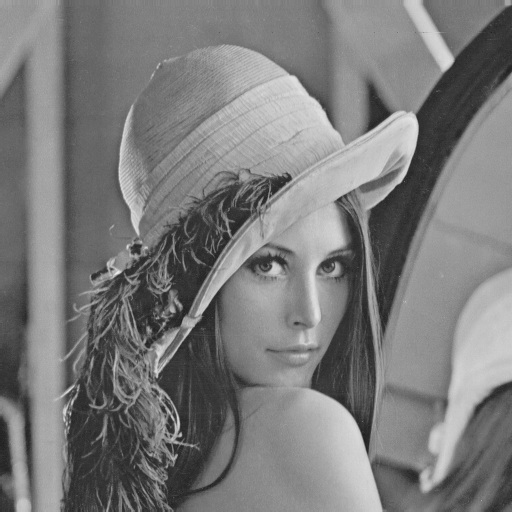
\includegraphics[keepaspectratio=true, scale=0.33]{images/lena.jpg}{}		
    }
    \hfill
    \subfloat[Magnitude representation\label{image-2:lena}]{
		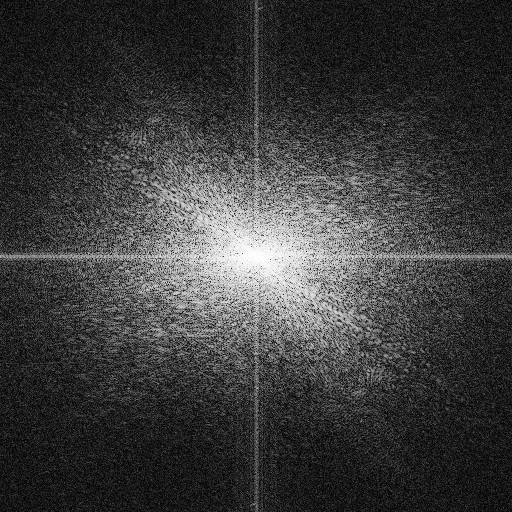
\includegraphics[keepaspectratio=true, scale=0.33]{images/lena_transformed.jpg}{}
    }
	\caption{Original image \ref{image-1:lena} transformed and represented with a quadrant shifted magnitude visualization (magnitude scale skewed for better visuals). \ref{image-2:lena}. }
    \label{fig:twodimentransform}
\end{figure}

The \gls{FFT} algorithm for two dimensional data, such as images, is first transformed row wise (each row as a separate sequence) and then a transform of each column. The implementation performs a row wise transformation and then transposes the whole image twice, see figure \ref{lst:cuda:host-2d-example}. A transformed image is shown in figure \ref{fig:twodimentransform}.

\begin{figure}[htbp]
	\centering
	\begin{framed}
		\includestandalone[width=\textwidth]{code/cuda-host-2d}	
	\end{framed}
	\caption{CUDA host code for the \gls{2D} \gls{FFT} algorithm.}
	\label{lst:cuda:host-2d-example}	
\end{figure}

The difference between the \gls{FFT} kernel for \gls{1D} and \gls{2D} are the indexing scheme. \gls{2D} are indexed as rows at \code{blockIdx.x} and columns at $\code{threadIdx.x} + \code{blockIdx.y} \cdot \code{blockDim.x}$. For \gls{2D} \code{blockIdx.z} is used as the sequence id in a batch.

\subsubsection{Transpose}

The transpose kernel uses a different index mapping of the 2D-data and blocks/threads then the \gls{FFT} kernel. The data is tiled in a grid pattern where each tile represents one block, indexed by \code{blockIdx.x} and \code{blockIdx.y}. The tile size is a multiple of 32 for both dimensions and limited to the size of the shared memory buffer, see table \ref{tab:threads-per-block} for specific size per technology. To avoid banking issues, the last dimension is increased with one but not used. However, resolving the banking issue have little effect on total running-time so when shared memory is limited to 32768, the extra column is not used. The tiles rows and columns are diveded over the \code{threadIdx.x} and \code{threadIdx.y} index respectively. See figure \ref{lst:cuda:device-transpose} for code example.

Shared memory example: The {\CU} shared memory can allocate 49152 bytes and a single data point require $\code{sizeof(float)} \cdot 2 = 8$ bytes. That leaves room for a tile size of $64 \cdot (64 + 1) \cdot 8 = 33280$ bytes.

\begin{figure}[H]
	\centering
	\begin{framed}
		\includestandalone[width=\textwidth]{code/cuda-device-transpose}	
	\end{framed}
	\caption{CUDA device code for the transpose kernel.}
	\label{lst:cuda:device-transpose}	
\end{figure}

The transpose kernel uses the shared memory and tiling of the image to avoid large strides through global memory. Each block represents a tile in the image. The first step is to write the complete tile to shared memory and synchronize the threads before writing to the output buffer. Both reading from the input memory and writing to the output memory is performed in close stride. Figure \ref{fig:transpose-memory} shows how the transpose is performed in memory.

\begin{figure}[H]
	\centering
	\includestandalone[width=\textwidth]{figures/transpose-tile}
	\caption{Illustration of how shared memory is used in transposing an image. Input data is tiled and each tile is written to shared memory and transposed before written to the output memory. }
	\label{fig:transpose-memory}
\end{figure}

\subsection{Differences}%
\subsubsection{Setup}%
The majority of differences in the implementations was related to the setup phase. The {\CU} implementation is the most straight forward, \code{cudaMalloc(...)} to allocate a buffer and \code{cudaMemcpy(...)} to populate it. With {\CU} you can write the device code in the same file as the host code and share functions. {\OCL} and {\GL} require a \code{char *} buffer and is most practical if written in seperate file and read as a file stream to a \code{char} buffer. {\DX} Shaders are most easily compiled from file. Figure \ref{fig:code:setup} demonstrates a simplified overview of how to setup the kernels in the different technologies.

\begin{figure}
	\centering
	\def \setupWidth {\textwidth / 2 - 20pt}	
	\subfloat[{\OCL} setup\label{setup:cu}]{		
		\fbox{\includestandalone[width=\setupWidth]{code/setup/cu}}
	}	
	\hfill
	\subfloat[{\OCL} setup\label{setup:ocl}]{		
		\fbox{\includestandalone[width=\setupWidth]{code/setup/ocl}}
	}
	\newline
	\subfloat[{\DX} setup\label{setup:dx}]{		
		\fbox{\includestandalone[width=\setupWidth]{code/setup/dx}}
	}
	\hfill
	\subfloat[{\GL} setup\label{setup:gl}]{		
		\fbox{\includestandalone[width=\setupWidth]{code/setup/gl}}
	}
	\caption{A overview of the setup functions for a kernel launch and buffer initialization.}
	\label{fig:code:setup}
\end{figure}

\subsubsection{Kernel execution}

Kernel execution in {\CU} is very much like any C-like language and the only difference is that the kernel launch syntax, $<<<$ and $>>>$, setting number of blocks and threads.

The other technologies require some more setup, {\OCL} and {\GL} set one parameter per line. {\OCL} maps with index whereas {\GL} maps with a string to the parameter. {\DX} is best suited to use a constant buffer for the parameters, the constant buffer is read only and accessible globally over the kernel. {\DX} and {\GL} share a similar launch style where the compute shader is set as the current program and then a dispatch call is made with the group (block) configuration. See table \ref{tab:kernel-execution} for a list of how the kernels are launched.

\begin{table}[H]
	\centering
	\includestandalone[width=\textwidth]{tables/kernel-execution}
	\caption{Table illustrating how to set parameters and launch a kernel.}
	\label{tab:kernel-execution}
\end{table}

\subsubsection{Kernel code}

This is the part where the code differ the least on but a few points. {\CU} have the strongest support for a {\CPP} -like language and only adds a function type specifier. The kernel program is accessible from the host via the \code{\_\_global\_\_} specifier. {\OCL} share much of this but restricted to a C99-style in the current version (2.0). One difference is how one can reference global and local buffers, these must be specified with the specifier \code{\_\_global} or \code{\_\_local}.

{\DX} and {\GL} Compute Shader is coded in \gls{HLSL} and \gls{GLSL} respectively. These languages are similar and share the same level of restrictions compared to CUDA C/C++ and {\OCL} C-code. Device functions can not use pointers or recursion. However these are of little importance for the performance since all code is in-lined in the compilation/building of the kernel program.

\subsubsection{Synchronization}

The synchronization of threads and blocks is slightly different, CUDA have the options to synchronize threads within a block and to synchronize host and device, the equivalent exists in all but {\DX} (DirectX 11) where the device synchronization is not done trivially as with a blocking function call. See table \ref{tab:kernel-synchronization} for the code used for each technology.

\begin{table}[H]
	\centering
	\includestandalone[width=\textwidth]{tables/kernel-synchronization}
	\caption{Synchronize functions regarding within blocks/groups and between host and device. CUDA, {\OCL} and {\DX} uses the same kernel stream to run them sequentially; {\GL} uses the command \code{glMemoryBarrier(GL\_SHADER\_STORAGE\_BARRIER\_BIT)} to ensure kernels are run in the same order as launched.}
	\label{tab:kernel-synchronization}
\end{table}

\section{Benchmark application CPU}

\subsection{FFT with OpenMP}

The {\OMP} implementation benefits in performance from calculating the twiddle factors in advance. The calculated values are stored in a buffer accessible from all threads. The next step is to calculate each stage of the \gls{FFT} algorithm. Last is the output index calculation where elements are reordered. See figure \ref{fig:omp:overview} for an overview.

\begin{figure}
	\centering
	\includestandalone[width=\textwidth]{figures/omp-overview}
	\caption{OpenMP implementation overview transforming sequence of size $N$.}
	\label{fig:omp:overview}
\end{figure}

\subsubsection{Twiddle factors}

The twiddle factor are stored for each butterfly operation. To save time, only the real part are calculated and the imaginary part is retrieved from the real parts due to the fact that $\sin(x) = \cos(\pi/2 + x)$ and $\sin(\pi/2 + x) = -\cos(x)$ to store. See figure \ref{tab:omp:twiddle-overview} for an example. The calculations will be split among the threads by static scheduling in two steps, first calculate the real values, secondly copy from real to imaginary.

\begin{table}[H]
	\centering
	\begin{tabular}{|l|l|r|}
	\multicolumn{3}{c}{Table $W$} \\ \hline
	$i$ & $\Re(W)$ & $\Im(W)$ \\ \hline
	0 & $\cos(\alpha \cdot 0)$ & $\Re(W[4])$ \\
	1 & $\cos(\alpha \cdot 1)$ & $\Re(W[5])$ \\
	2 & $\cos(\alpha \cdot 2)$ & $\Re(W[6])$ \\
	3 & $\cos(\alpha \cdot 3)$ & $\Re(W[7])$ \\	
	4 & $\cos(\alpha \cdot 4)$ & $-\Re(W[0])$ \\
	5 & $\cos(\alpha \cdot 5)$ & $-\Re(W[1])$ \\
	6 & $\cos(\alpha \cdot 6)$ & $-\Re(W[2])$ \\
	7 & $\cos(\alpha \cdot 7)$ & $-\Re(W[3])$ \\ \hline
\end{tabular}
	\caption{Twiddle factors for a 16-point sequence where $\alpha = (2 \cdot \pi) / 16$. Each row $i$ corresponds to the $i$th butterfly operation.}
	\label{tab:omp:twiddle-overview}
\end{table}

\subsubsection{Butterfly}

The same butterfly operation uses the constant geometry index scheme. The indexes are not stored from one stage to the next but it makes the output come in continues order. The butterfly operations are split among the threads by static scheduling.

\subsubsection{Bit Reversed Order}

See figure \ref{fig:omp:bit-reverse-order} for code showing the bit reverse ordering operation in C/C++ code.

\begin{figure}[H]
	\centering
	\begin{framed}
		\includestandalone[width=\textwidth]{code/omp-bit-reverse}	
	\end{framed}
	\caption{ C/C++ code performing the bit reverse ordering of a N-point sequence. }
	\label{fig:omp:bit-reverse-order}
\end{figure}

\subsection{FFT 2D with OpenMP}

The implementation of \gls{2D} \gls{FFT} with {\OMP} run the transformations row wise and transposes the image and repeat. The twiddle factors are calculated once and stays the same.

\subsection{Differences with GPU}

The OpenMP implementation differs from the \gls{GPU} with the fact that twiddle factors are pre computed and it uses the constant geometry implementation in all stages. The amount of parallel threads are on the {\INTELCPU} four whereas on the \gls{GPU} in the order of up to 192 (seven warps, one per \gls{SM}, with 32 threads each). This highly effects performance when the size of the problem grows.

\section{Benchmark configurations}

\subsection{Limitations}

All implementations are limited to handle sequences of $2^n$ length or $2^m \times 2^m$ where $n$ and $m$ are integers with maximal value of $n = m + m = 26$. The selected \gls{GPU}s have a maximum of 2GB global memory available. The limitation is required since the implementation uses a total of $2^{26} \cdot \code{sizeof(float2)} \cdot 2 = 1073741824$ bytes. However on the {\AMDCARD} card, problems with {\DX} and {\GL} set the limit lower. {\DX} handled sizes of $n <= 2^{24}$ and {\GL} $n <= 2^{24}$ and $m <= 2^{9}$.

\subsection{Testing}

All tests executed on the \gls{GPU} utilize some implementation of event time stamps. The time stamp event retrieve the actual start of the kernel if the current stream is busy. The \gls{CPU} implementations used Windows \emph{QueryPerformanceCounter} function, which is a high resolution ($<1{\micro}s$) time stamp.

\subsection{Reference libraries}

A reference libraries per platform was included to compare how well the FFT implementation performed. The \emph{\FFTW} library for the \gls{CPU}, runs a planning scheme to create an execution plan for each environment and data input size. Similar strategy is used in the {\CUFFT} and {\CLFFT} libraries used for the {\NVCARD} and {\AMDCARD} respectively. Table \ref{tab:external-implementations} sums up information about the external libraries.

\begin{table}
	\centering
	\begin{tabular}{|l|l|l|l|}
	\hline
	Platform & Model & Library name & Version \\ \hline
	NVIDIA GPU & GeForce GTX 670 & cuFFT & TODO \\
	AMD GPU & Radeon R7 260X & clFFT & 2.8.0 \\ \hline
	Intel CPU & Core i7 3770K 3.5GHz & FFTW & 3.3.4 \\ \hline
\end{tabular}
	\caption{Libraries included to compare with the implementation.}
	\label{tab:external-implementations}
\end{table}%
\chapter{Results and Evaluation}

\todo{Write short explanation of this chapter.}

\section{Performance}

\todo{Present all performance comparisons.}

\begin{figure}
	\centering
	\includestandalone[width=\textwidth]{plots/gtx670/1d}
	\caption{Plot showing 1D FFT on GTX 670}
	\label{fig:gtx:1d}
\end{figure}

\section{Qualitative assessment}

\todo{Present some soft values.}

\subsection{Scalability}

\todo{Present how well problems scale.}

\subsection{Portability}

\todo{Present how well code is ported to other platforms.}

\subsection{Programmability}

\todo{Present how easy or hard an algorithm is to implement.}
%
%
\backmatter%
%
\bibliography{IEEEfull,IEEEabrv,custom_library}%
%
\printindex%
%
\end{document}%